\documentclass[xcolor=pdftex,x11names,table,hyperref]{beamer}

\usepackage{verbatim}
\usepackage{setspace}
\usepackage{graphbox}
\usepackage{url}
\usepackage{xcolor} % See documentation PDF at http://www.ctan.org/pkg/xcolor
\definecolor{darkgreen}{rgb}{0,0.3,0}
\definecolor{darkblue}{rgb}{.05,.05,.30}
\definecolor{lightgrey}{rgb}{0.65,0.65,0.65}
\usepackage{tikzsymbols}
\usetikzlibrary{matrix,arrows,positioning,automata,shadows,shapes.geometric,shapes.misc}


\setbeamertemplate{section in toc}[sections numbered]
\setbeamertemplate{subsection in toc}[subsections numbered]
\setbeamertemplate{subsubsection in toc}[subsubsections numbered]
\usetheme{Singapore}
\setbeamertemplate{navigation symbols}{}
\setbeamertemplate{footline}{%
\vspace{0.0em}%
\hspace{0.5em}%
{\color[rgb]{.1,.1,.1} \insertframenumber{}~/~\inserttotalframenumber}
}

\newcommand{\code}[1]{{\color{darkgreen}\texttt{#1}}}
\newcommand{\detail}[1]{{\color{lightgrey}\small{}#1}}
\newcommand{\teeny}[1]{\scalebox{0.17}{#1}}
\newcommand{\tablecolors}{\rowcolors{2}{blue!12}{white}} % Cool table colors

\newcommand{\actfun}[1]{\includegraphics[height=0.11\textheight,align=c]{images/#1}} % For consistency

\begin{document}

\title{Neural Networks \\[1.5em]
 %
\includegraphics[width=0.5\textwidth]{images/kitten_string_flickr_albaraa.jpg} \\[-1.0em]
 \small{Part 2} \\[1.0em]
 Normalization Speedups and Processing Sequential Data \\[1.0em]
 }
\author{\href{http://jon.dehdari.org}{Jon Dehdari} and \href{http://www.coli.uni-saarland.de/~asayeed/}{Asad Sayeed}}
\frame{\titlepage}

\begin{frame}{Good Morning!}
	\begin{center}
	
\includegraphics[height=0.55\textheight]{images/skel_nn.jpg}
	\end{center}
\end{frame}


\begin{frame}{First things first}
  \begin{itemize}
  \item Just want to know: how well do we remember our matrix multiplication?\pause
  \item Or linear algebra?\pause
  \item Then when we intone this:
    \begin{center}
    tanh($W\mathbf{x} + \mathbf{b}$)
    \end{center}
    We all get what it means?\pause
  \item And do we remember what regression actually is?\pause
  \item When I say ``train a model'', do we all know what training an NN really ``means''?\pause
  \end{itemize}

  \begin{center}
    \textbf{OK, great, I just wanted to make sure we're on the same page}
  \end{center}

\end{frame}

\begin{frame}{Second things second}

  \begin{itemize}
  \item OK, now that we have {\it that} out of the way, remember softmax?
  \end{itemize}
  \begin{align}
    % \hspace*{-5.5em}%
    P(y | \mathbf{x}) & = \frac{{\mathnormal e}^{\boldsymbol W_y \cdot \mathbf{x}} }{Z} \hspace*{0.4em} \substack{\color{green}{ \leftarrow \, \text{\parbox[c]{0.58\textwidth}{ {\footnotesize \, exponentiation helps ensure scores are positive}}}} \\[1.0em]  \color{green}{ \leftarrow \, \text{\parbox[c]{0.55\textwidth}{ \textbf{normalization constant}, {\footnotesize to ensure the \\[-0.9em] score of all possible outcomes sums to 1}}}}}  \nonumber\\[1.0em]
    % & = \frac{1}{Z} {\mathnormal e}^{\boldsymbol W_y \cdot \mathbf{x}}  \nonumber\\[1.0em]
                      & =     \frac{{\mathnormal e}^{\boldsymbol W_y \cdot \mathbf{x}}}{\sum_h {\mathnormal e}^{\boldsymbol W_h \cdot \mathbf{x}}}  \,\, \substack{ \, \\[1.0em]  \color{green}{ \leftarrow \text{\parbox[c]{0.50\textwidth}{ \, to get Z, we just add up scores from \\[-0.8em] all possible outcomes}}}} \nonumber\\[1.0em]
                      & = \text{softmax}(\boldsymbol W_y \cdot \mathbf{x}) \nonumber%\\[1.0em]
                      % & =  \nonumber\\[1.0em]
  \end{align}\pause
  \begin{itemize}
  \item What does it mean?\pause
  \item But there's a problem\ldots
  \end{itemize}        
\end{frame}

% automatic differentiation of graph, why it's nice
%\begin{frame}{}
%\begin{itemize}
%	\item 
%	\item 
%\end{itemize}
%\end{frame}

% discussion of softmax, class-based decomp, hier softmax
\begin{frame}\frametitle{Softmax Normalization}

% http://tex.stackexchange.com/a/54007
\begin{minipage}[0.8\textheight]{\textwidth}
\begin{columns}[T]
\begin{column}{0.6\textwidth}
\begin{itemize}
	\item The slowest part of training a neural net LM is softmax normalization
	\item Why?  Before the softmax layer (final layer) we just have a real number, not a probability
	\item So we need to know the sum of scores for all possible words being predicted (ie. the normalization constant)
\end{itemize}
\end{column}
\begin{column}{0.6\textwidth}
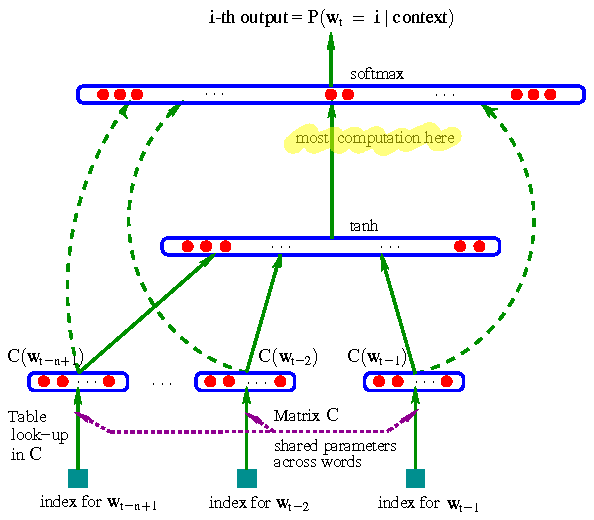
\includegraphics[width=1.0\textwidth]{images/bengio-etal2003_pg6_image_alt2.pdf}
\end{column}
\end{columns}
\end{minipage}

\pause

\hspace*{-2.5em}%
\begin{minipage}{1.0\textwidth}
\begin{itemize}
	\item This involves $|V|$ steps, where $|V|$ is the size of the vocabulary
	\item Typical values of $|V|$ are between 10K to 10M
	\item We must do this for every word in our training set (eg.\ 1M--1B), every epoch ($>10$)
\end{itemize}
\end{minipage}

\end{frame}


\begin{frame}{Speeding Up Normalization}
\begin{itemize}[<+->]
	\item Can we speed up normalization? We can approximate $Z$\,:
	\item \textbf{Class-based Decomposition} works like class-based LMs: first determine prob.\ of a given word's class/POS, then the prob.\ of the specific word \detail{$\mathcal{O} ( \sqrt{|V|} )$}
	\item \textbf{Hierarchical Softmax} extends this idea to a fully binary-branching hierarchy of the vocabulary (like an ontology) \detail{$\mathcal{O} (\log_2(|V|) ) $ }
	\item \textbf{Noise Contrastive Estimation} (NCE) disposes with MLE (in Softmax).  Instead, a binary classifier is learned: observed training data vs.\ artificially generated noise.  word2vec's negative sampling is a simplified version. \detail{$\mathcal{O} (1) $}
	\item \textbf{Self Normalization} ensures that the normalization constant $Z$ is close to one. Slow for training, fast for test-time queries
\end{itemize}
\end{frame}

% Second set: recurrent NN's (Elman (vanishing/exploding gradient), GRU, LSTM), BPTT, maybe convolutional nets
% http://deeplearning.net/tutorial/lstm.html
% http://arxiv.org/pdf/1412.3555v1.pdf
% https://colah.github.io/posts/2015-08-Understanding-LSTMs/
% https://www.tensorflow.org/versions/master/tutorials/recurrent/index.html#recurrent-neural-networks
% https://www.ling.ohio-state.edu/~jonsafari/teaching/uds/lm/pres_09_rnnlm.pdf
% http://keras.io/layers/recurrent/
% https://en.wikipedia.org/wiki/LSTM

\begin{frame}{Neural Networks for Sequential Data}
\begin{itemize}
	\item Feedforward (FF) networks only indirectly deal with sequential data (like language)
	\item FF Neural LMs are basically `soft' $n$-gram LMs -- their history is still fixed
	\pause
	\item The model needs to `remember' a longer history, with loops
\end{itemize}

%\begin{center}
%\begin{tiny}
%%\usepackage[hyperref,table,x11names]{xcolor} % See documentation PDF at http://www.ctan.org/pkg/xcolor
%\usetikzlibrary{matrix,arrows,positioning,automata,shadows,shapes.geometric,shapes.misc}
\definecolor{darkblue}{rgb}{.05,.05,.30}
\definecolor{darkgreen}{rgb}{.05,.30,.05}
\definecolor{darkred}{rgb}{.30,.05,.05}

\hspace*{-3em}%
 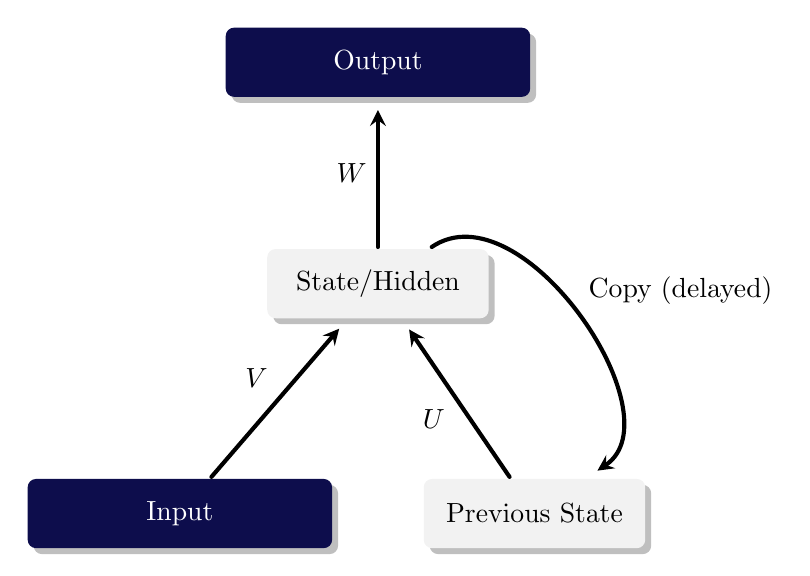
\begin{tikzpicture}[->, >=stealth, line cap=round, shorten >=.4em, auto, node distance=8.0em, semithick, initial text={},]
   \tikzstyle{every state}=[rounded corners=.3em, rectangle, fill=darkblue, draw=none, text=white, drop shadow, minimum width=11em, hidden/.style ={white!95!black,text=black,minimum width=8em},]
   \tikzstyle{every path}=[line width=.15em]

   \node[state] (output_orig) {Output};
   \node[state,hidden] (hidden_orig) [below of=output_orig] {State/Hidden};
   \node[state] (input_orig) [below left=8em of hidden_orig.south east] {Input};
   \node[state,hidden] (previous) [below right=8em of hidden_orig.south west] {Previous State};


   \path


  (hidden_orig)
    edge [] node {$W$} (output_orig)
  (input_orig)
    edge [] node {$V$} (hidden_orig)
  (previous)
    edge [] node {$U$} (hidden_orig)
  (hidden_orig)
    edge [bend left=90] node {Copy (delayed)} (previous)
   ;
 \end{tikzpicture}

%\end{tiny}
%\end{center}
\end{frame}


\begin{frame}{Recurrent Neural Networks}
\hspace*{-1.0em} A neural net with loops is called \textbf{recurrent} \\[1.0em]
\pause

\hspace*{-3.0em}%
\begin{tabular}{p{.63\textwidth}p{.4\textwidth}}
\begin{minipage}{0.6\textwidth}
\begin{itemize}
	\item The current hidden layer of the model is based on both the current word and the hidden layer of the previous timestep
	\item This is implemented by copying the hidden layer to another layer, overwriting the existing weights
	\item This specific RNN is called an \textbf{Elman network} (or \textbf{simple RNN} / SRN)
\end{itemize}
\end{minipage}
 & 
%\begin{scalebox}{0.6}{%
\begin{minipage}{1.0\textwidth}
\begin{tiny}
%\usepackage[hyperref,table,x11names]{xcolor} % See documentation PDF at http://www.ctan.org/pkg/xcolor
%\usetikzlibrary{matrix,arrows,positioning,automata,shadows,shapes.geometric,shapes.misc}
\definecolor{darkblue}{rgb}{.05,.05,.30}
\definecolor{darkgreen}{rgb}{.05,.30,.05}
\definecolor{darkred}{rgb}{.30,.05,.05}

\hspace*{-3em}%
 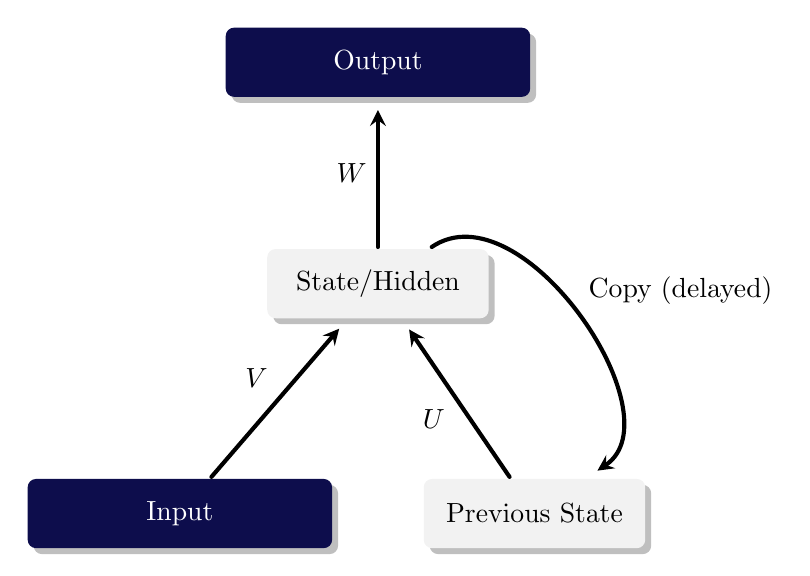
\begin{tikzpicture}[->, >=stealth, line cap=round, shorten >=.4em, auto, node distance=8.0em, semithick, initial text={},]
   \tikzstyle{every state}=[rounded corners=.3em, rectangle, fill=darkblue, draw=none, text=white, drop shadow, minimum width=11em, hidden/.style ={white!95!black,text=black,minimum width=8em},]
   \tikzstyle{every path}=[line width=.15em]

   \node[state] (output_orig) {Output};
   \node[state,hidden] (hidden_orig) [below of=output_orig] {State/Hidden};
   \node[state] (input_orig) [below left=8em of hidden_orig.south east] {Input};
   \node[state,hidden] (previous) [below right=8em of hidden_orig.south west] {Previous State};


   \path


  (hidden_orig)
    edge [] node {$W$} (output_orig)
  (input_orig)
    edge [] node {$V$} (hidden_orig)
  (previous)
    edge [] node {$U$} (hidden_orig)
  (hidden_orig)
    edge [bend left=90] node {Copy (delayed)} (previous)
   ;
 \end{tikzpicture}

\end{tiny}
\end{minipage}
%}
\end{tabular} \\[1.0em]


\hspace*{-2.5em}%
\begin{minipage}{1.0\textwidth}
\begin{itemize}
	\item To train an RNN, we first need to `unroll' the loops
\end{itemize}
\end{minipage}
\end{frame}



\begin{frame}{Training RNNs with BPTT}
\begin{itemize}
	\item Backpropagation through time (BPTT) trains RNNs by unrolling the most recent part of the loop
	\item Now the network is feedforward
	\item {\small Below is an example of an unrolled RNN using last 3 states \detail{($\tau = 3$)} }
\end{itemize}

\vspace*{0.5em}

\begin{tiny}
\scalebox{0.94}{%
%\usepackage[hyperref,table,x11names]{xcolor} % See documentation PDF at http://www.ctan.org/pkg/xcolor
%\usetikzlibrary{matrix,arrows,positioning,automata,shadows,shapes.geometric,shapes.misc}
\definecolor{darkblue}{rgb}{.05,.05,.30}
\definecolor{darkgreen}{rgb}{.05,.30,.05}
\definecolor{darkred}{rgb}{.30,.05,.05}

\hspace*{-3em}%
 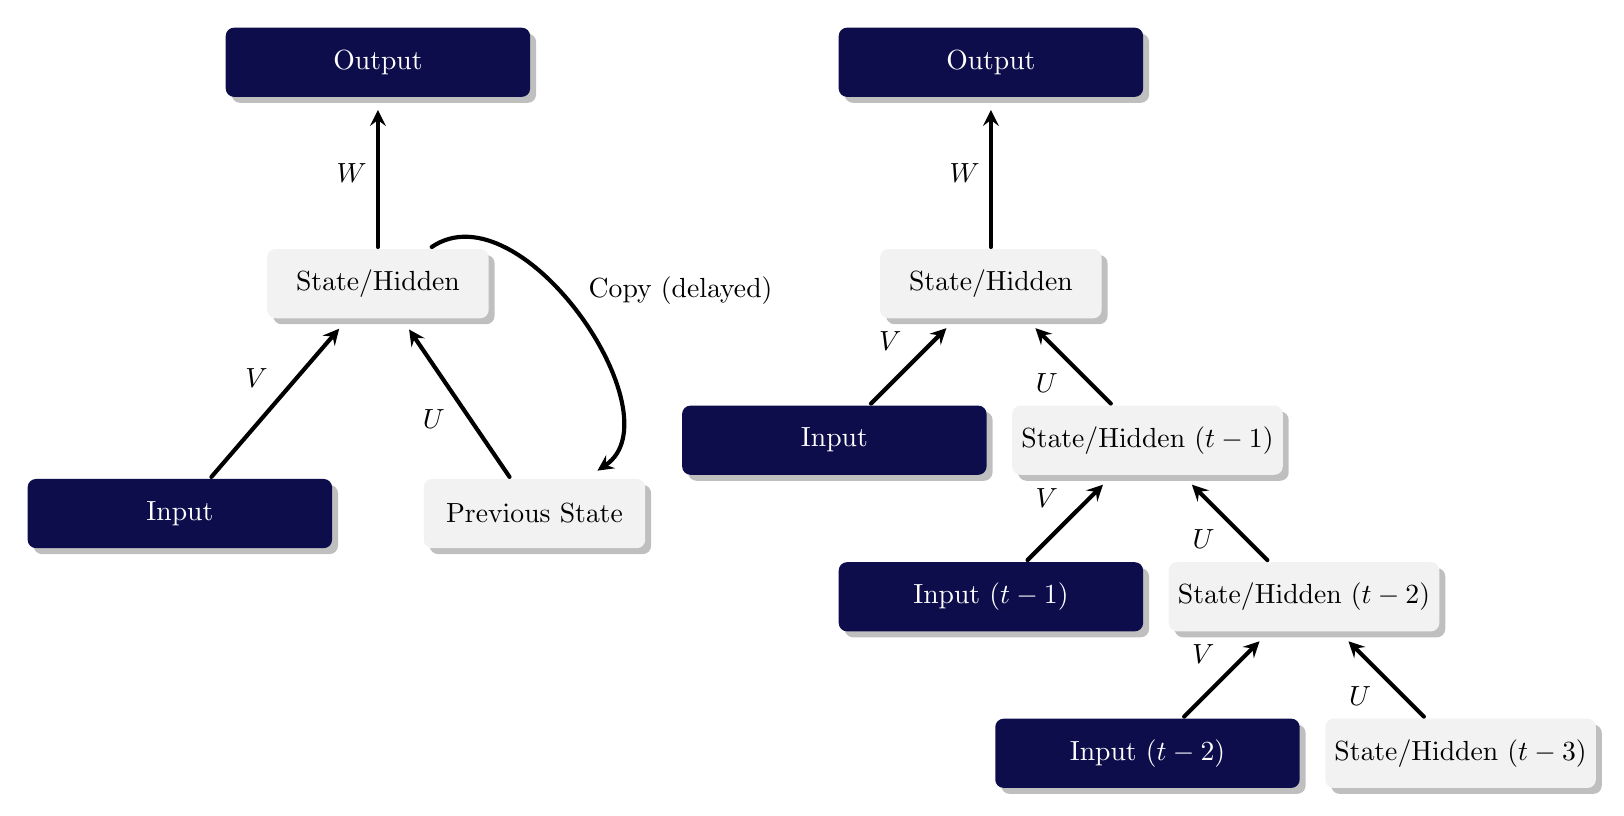
\begin{tikzpicture}[->, >=stealth, line cap=round, shorten >=.4em, auto, node distance=8.0em, semithick, initial text={},]
   \tikzstyle{every state}=[rounded corners=.3em, rectangle, fill=darkblue, draw=none, text=white, drop shadow, minimum width=11em, hidden/.style ={white!95!black,text=black,minimum width=8em},]
   \tikzstyle{every path}=[line width=.15em]

   \node[state] (output) {Output};
   \node[state,hidden] (hidden) [below of=output] {State/Hidden};
   \node[state] (input) [below left of=hidden] {Input};
   \node[state,hidden] (hidden_t-1) [below right of=hidden] {State/Hidden ($t-1$)};
   \node[state] (input_t-1) [below left of=hidden_t-1] {Input ($t-1$)};
   \node[state,hidden] (hidden_t-2) [below right of=hidden_t-1] {State/Hidden ($t-2$)};
   \node[state] (input_t-2) [below left of=hidden_t-2] {Input ($t-2$)};
   \node[state,hidden] (hidden_t-3) [below right of=hidden_t-2] {State/Hidden ($t-3$)};

   \node[state] (output_orig) [left=11.0em of output.west] {Output};
   \node[state,hidden] (hidden_orig) [below of=output_orig] {State/Hidden};
   \node[state] (input_orig) [below left=8em of hidden_orig.south east] {Input};
   \node[state,hidden] (previous) [below right=8em of hidden_orig.south west] {Previous State};


   \path

  (hidden)
    edge node {$W$} (output)
  (input)
    edge node {$V$} (hidden)
  (hidden_t-1)
    edge node {$U$} (hidden)
  (input_t-1)
    edge node {$V$} (hidden_t-1)
  (hidden_t-2)
    edge node {$U$} (hidden_t-1)
  (input_t-2)
    edge node {$V$} (hidden_t-2)
  (hidden_t-3)
    edge node {$U$} (hidden_t-2)

  (hidden_orig)
    edge [] node {$W$} (output_orig)
  (input_orig)
    edge [] node {$V$} (hidden_orig)
  (previous)
    edge [] node {$U$} (hidden_orig)
  (hidden_orig)
    edge [bend left=90] node {Copy (delayed)} (previous)
   ;
 \end{tikzpicture}

}
\end{tiny}
\end{frame}


\begin{frame}{Problems with Elman Networks / SRNs}
\begin{itemize}
	\item The main problem with Elman networks (SRNs) is that gradients less than 1 become exponentially small over time (the \textbf{vanishing gradient problem}) ...
	\item and gradients greater than 1 become exponentially large over time (the \textbf{exploding gradient problem})$^{^*}$
	\item This leads to instability, and bad results
	\pause
	\item What if we had another neural network help the first network learn long-distance relationships?
	\pause
	\item That's basically what we do when we add more weight matrices to a neural network
	\pause
	\item As you might guess, that's what we're going to do ...
\end{itemize}
\vspace*{5.0em}
\teeny{$^*$\,The exploding gradient problem can be alleviated by clipping large gradient values to some maximum number.}
\end{frame}


\begin{frame}{Long Short-term Memory}
\begin{center}
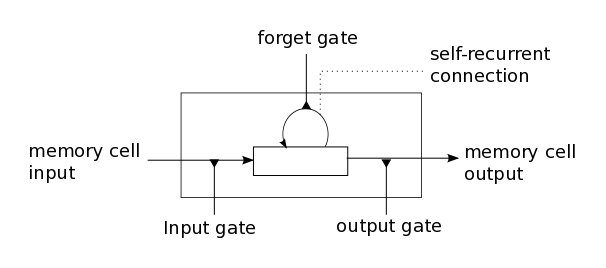
\includegraphics[width=0.55\textwidth]{images/lstm_memorycell.png}
\end{center}
\vspace*{-2.0em}

\begin{itemize}
	\item A \textbf{long short-term memory} (LSTM) network adds more weight matrices to function as \emph{soft} `memory gates', so that long-distance phenomena in our data can be held in the network over multiple timesteps
	\pause
	\item Input gate: $i_t = \sigma(W_i x_t + U_i h_{t-1} + b_i) $
	\item Candidate memory state: $ \tilde{C}_t = \text{tanh}( W_c x_t + U_c h_{t-1} + b_c ) $
	\item Forget gate: $ f_t = \sigma( W_f x_t + U_f h_{t-1} + b_f ) $
	\item Memory state: $ C_t = i_t \odot \tilde{C}_t + f_t \odot \tilde{C}_{t-1} $
	\item Output gate: $ o_t = \sigma(W_o x_t + U_o h_{t-1} + V_o C_t + b_o) $
	\item Output: $ h_t = o_t \odot \text{tanh}(C_t) $
\end{itemize}
\teeny{Image courtesy of a nice tutorial at \url{http://deeplearning.net/tutorial/lstm.html}.  Another nice tutorial is at \url{https://colah.github.io/posts/2015-08-Understanding-LSTMs}.  The symbol $\odot$ is the Hadamard product (a.k.a.\ elementwise multiplication), which just multiplies corresponding elements of two matrices and returns another matrix of their products.}
\end{frame}

\begin{frame}{LSTM - anatomy}
  \begin{center}
    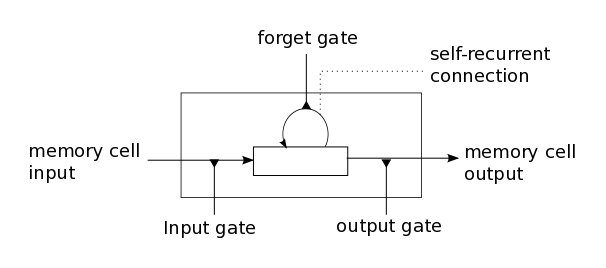
\includegraphics[width=0.55\textwidth]{images/lstm_memorycell.png}
  \end{center}
  
  \begin{itemize}
  \item Input gate: $i_t = \sigma(W_i x_t + U_i h_{t-1} + b_i) $
    \begin{itemize}
    \item Sigmoid - between 0 and 1, used to weight importance of input. 
    \item $x_t$ current input, $h_{t-1}$ previous hidden state.      
    \end{itemize}\pause
  \item Candidate memory state: $ \tilde{C}_t = \text{tanh}( W_c x_t + U_c h_{t-1} + b_c ) $
    \begin{itemize}
    \item What the cell should remember given current input and previous hidden state, other things being equal
    \item tanh makes it between -1 and 1.
    \end{itemize}\pause
  \item Now come the fun parts.
  \end{itemize}
\end{frame}
  

\begin{frame}{LSTM - anatomy}
  \begin{center}
    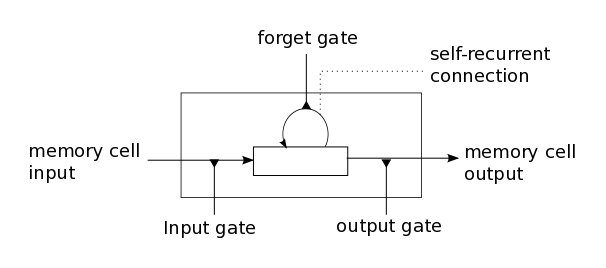
\includegraphics[width=0.55\textwidth]{images/lstm_memorycell.png}
  \end{center}
  
  \begin{itemize}
  \item Forget gate: $ f_t = \sigma( W_f x_t + U_f h_{t-1} + b_f ) $
    \begin{itemize}
    \item Sigmoid - between 0 and 1, used to weight how much we're going to discount current memory state. 
    \item $x_t$ current input, $h_{t-1}$ previous hidden state.      
    \item (Weights have to be learned for each gate type!)
    \end{itemize}\pause
  \item Memory state: $ C_t = i_t \odot \tilde{C}_t + f_t \odot \tilde{C}_{t-1} $	
    \begin{itemize}
    \item What the cell is going to remember, given the discount of the forget gate of the previous memory state.
    \end{itemize}
  \end{itemize}
\end{frame}

\begin{frame}{LSTM - anatomy}
  \begin{center}
    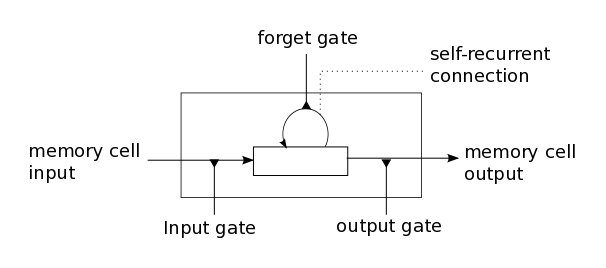
\includegraphics[width=0.55\textwidth]{images/lstm_memorycell.png}
  \end{center}
  
  \begin{itemize}
  \item Output gate: $ o_t = \sigma(W_o x_t + U_o h_{t-1} + V_o C_t + b_o) $ 
    \begin{itemize}
    \item Now includes weights not only on $x_t$ and $h_{t-1}$, but also $C_t$ -- ie, how much the 
      new memory state contributes to the next cell.
    \end{itemize}\pause
  \item Output: $ h_t = o_t \odot \text{tanh}(C_t) $ - then emit the new state for the next cell
  \end{itemize}\pause
  And then it's all a matter of training, simple, right?
\end{frame}

\begin{frame}{Gates}
\begin{center}
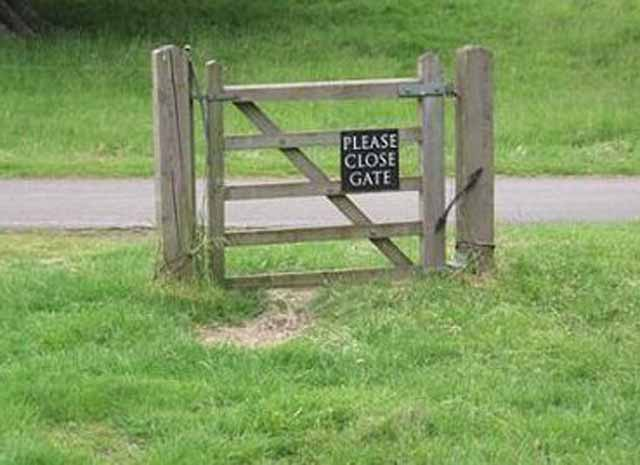
\includegraphics[height=0.30\textheight]{images/gate_funny.jpg}
\hspace{1.7em}

\includegraphics[height=0.30\textheight]{images/bill-gates-pie.jpg}
\end{center}
%\vspace*{-0.8em}

\hspace*{-1.0em}%
\begin{minipage}{1.1\textwidth}
\begin{itemize}[<+->]
	\item Each soft gate that we use is just another weight matrix that we apply to various inputs, then squash through a logistic function
	\item For example, if the value of the forget gate $f$ is 0, the memory state from the previous timestep ($C_{t-1}$) is completely forgotten
	\item If $f=1$, we fully keep the memory state of the previous timestep
	\item The value of $f$ can be between 0 and 1, so the memory decays
	\item That's a big difference over Elman networks / SRNs
\end{itemize}
\end{minipage}
\teeny{\scalebox{0.2}{Image ostensibly from \url{http://www.amusingtime.com/funny/funny-signs/page/209}}}
\end{frame}

% see figure 1 in http://arxiv.org/abs/1603.05118
\begin{frame}{Gated Recurrent Units (GRUs)}
\begin{center}
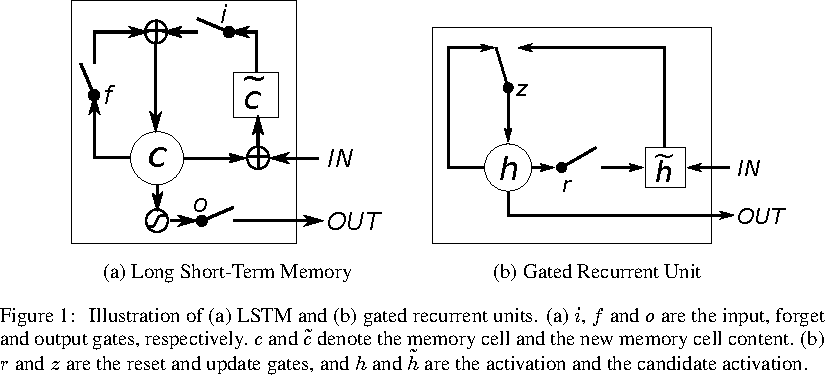
\includegraphics[width=0.75\textwidth]{images/chung-etal2014_fig1.pdf}
\end{center}
\vspace*{-1.0em}

\begin{itemize}
	\item \textbf{Gated recurrent units} (GRUs) are very similar to LSTMs, but are a little simpler
	\item GRUs merge the forget and input gates into a single update gate
	\item GRUs also merge the hidden state and the cell state
	\item Both LSTMs and GRUs achieve similar performance on many tasks
\end{itemize}
\teeny{Image courtesy of \url{http://arxiv.org/pdf/1412.3555v1.pdf}}
\end{frame}


\begin{frame}{Rube Goldberg Network}
\begin{center}
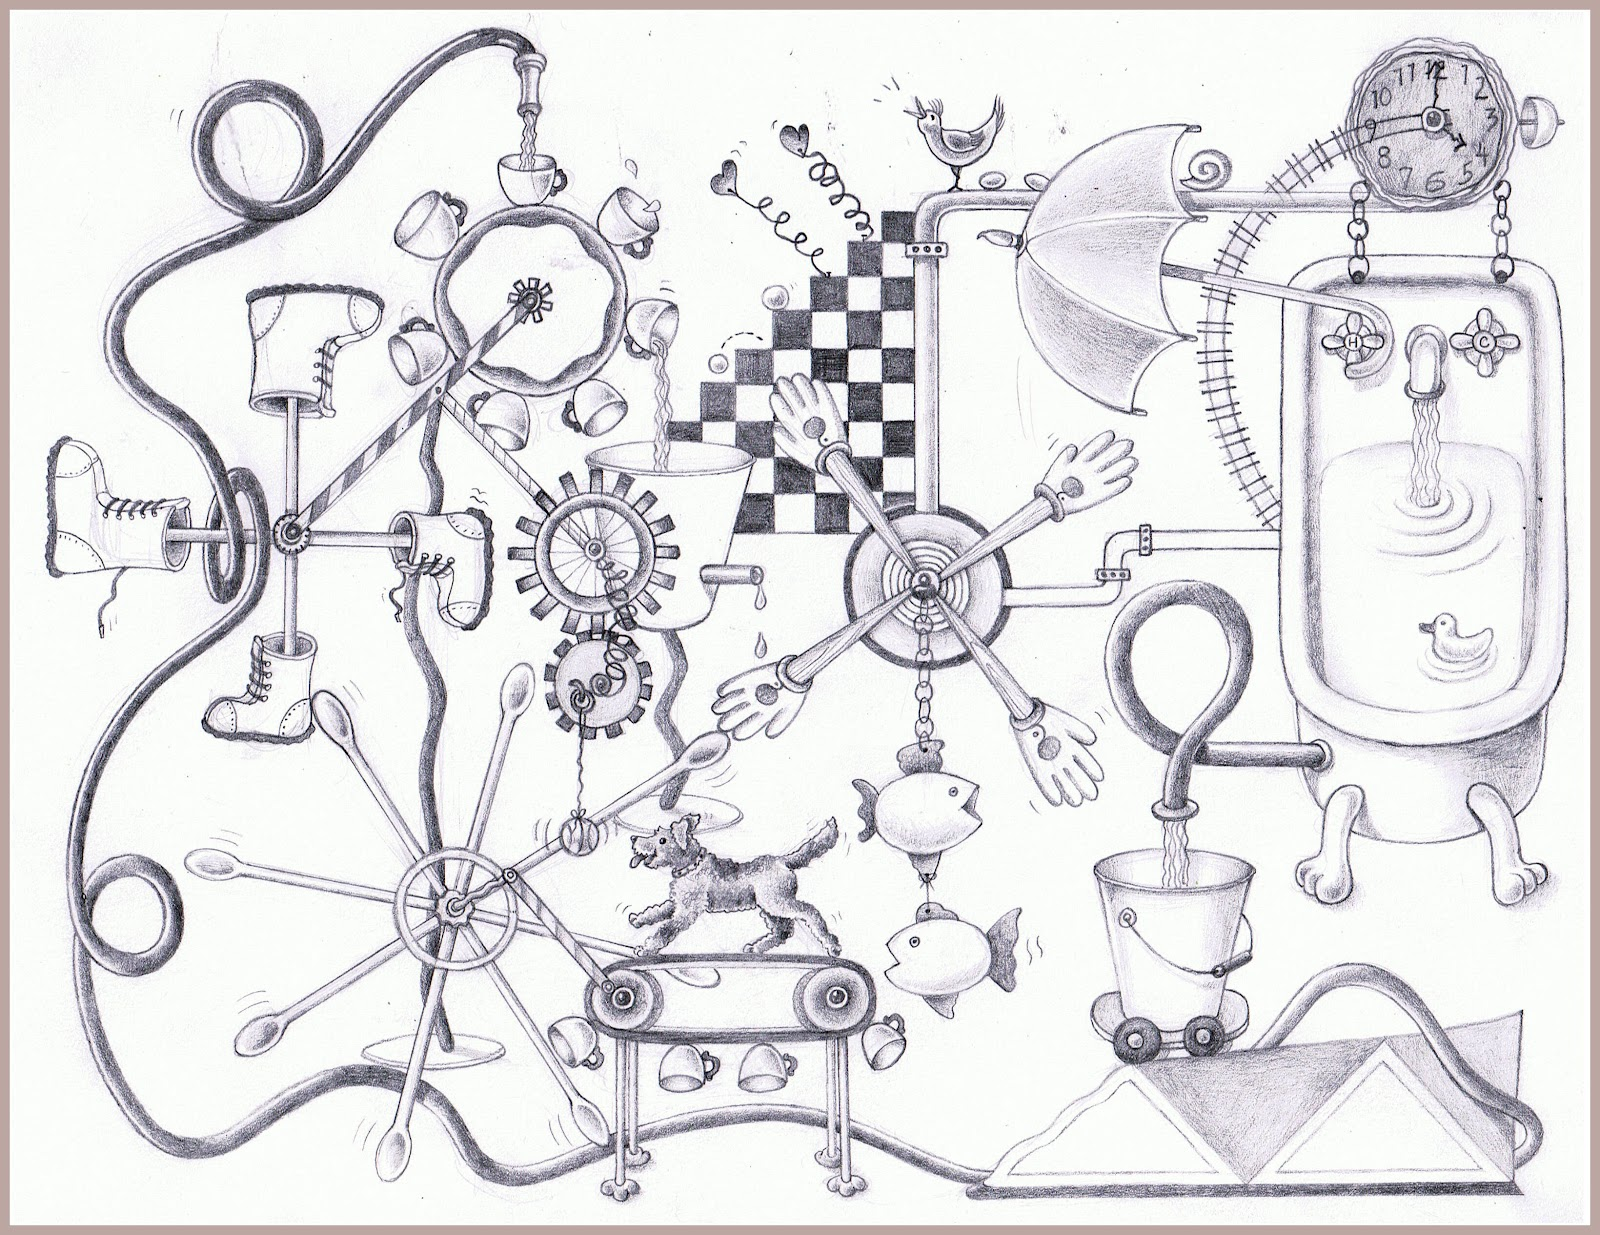
\includegraphics[width=0.85\textwidth]{images/rube_goldberg_machine.jpg}
\end{center}

%It's all starting to sound like a \href{https://en.wikipedia.org/wiki/Rube_Goldberg_machine}{Rube Goldberg machine}!
\end{frame}

\begin{frame}{Further Reading}

\textbf{Overviews}: \\[0.5em]
\begin{minipage}{1.1\textwidth}
\begin{tiny}
\begin{itemize}
	\item \url{https://www.reddit.com/r/MachineLearning/comments/44bxdj/scrn\_vs\_lstm/czp4hqr/}
	\item \url{https://colah.github.io/posts/2015-08-Understanding-LSTMs/}
	\item \url{https://medium.com/@shiyan/understanding-lstm-and-its-diagrams-37e2f46f1714}
	\item \url{http://deeplearning.net/tutorial/lstm.html}
	\item \url{http://arxiv.org/abs/1412.3555}
	\item \url{https://www.tensorflow.org/versions/master/tutorials/recurrent/index.html\#recurrent-neural-networks}
	\item \url{http://keras.io/layers/recurrent/}
	\item \url{https://drive.google.com/open?id=0B-aFax-9-qt3Sllodkpmc1M0MUk}
	\item \url{https://en.wikipedia.org/wiki/LSTM}
\end{itemize}
\end{tiny}
\end{minipage}

\vspace{1.0em}
\textbf{Original Papers}:
\begin{tiny}
\begin{description}
	\item[SRN] Elman, Jeffrey L. 1990. \href{http://citeseerx.ist.psu.edu/viewdoc/summary?doi=10.1.1.28.9476}{Finding Structure in Time}. \textit{Cognitive Science} 14.179--211.
	\item[LSTM] Hochreiter, Sepp, and J\"{u}rgen Schmidhuber. 1997. \href{http://deeplearning.cs.cmu.edu/pdfs/Hochreiter97_lstm.pdf}{Long Short-Term Memory}. \textit{Neural Computation} 9.1735--1780.
	\item[GRU] Kyunghyun Cho, Bart van Merri\"{e}nboer, \c{C}a\u{g}lar G\"{u}l\c{c}ehre, Fethi Bougares, Holger Schwenk, and Yoshua Bengio. 2014. \href{https://arxiv.org/abs/1406.1078}{Learning phrase representations using RNN encoder-decoder for statistical machine translation}. In \textit{Proceedings of the Empiricial Methods in Natural Language Processing (EMNLP 2014)}.
\end{description}
\end{tiny}
\end{frame}


% \begin{frame}{}
% \begin{itemize}
% 	\item 
% 	\item 
% 	\item 
% \end{itemize}
% \end{frame}


\end{document}
